\subsection{Studies in the Uniform Phase Space} % (fold)
\label{sub:flat_hypercube_studies}

Since we outperform physics-derived variables, we would like to know where these performance improvements come from. Our first approach to this is \emph{hypercube reweighting}. In particular, we derive weights such that the joint distributions of mass, $n$-subjettiness, and $p_T$ are non-discriminative. Specifically, we require

\begin{equation}
  f(m, \tau_{21}, p_T| W'\rightarrow WZ) \approx f(m, \tau_{21}, p_T| QCD).
\end{equation}

We then take our globally trained neural network (Figure~\ref{fig:combinedROC}) and apply the discriminant under this ``flattening'' transformation. We also use the training weights inside this window and train an additional CNN. In particular, we look for increases in performance, which would indicate information learned beyond physics variables since we removed the discrimination power using hypercube weighting.

In Figure~\ref{fig:rocCube} we show that the globally trained NN retains discrimination power even once we ``subtract'' the discrimination power of primitives from physics.

\begin{figure}[htbp]
  \centering
  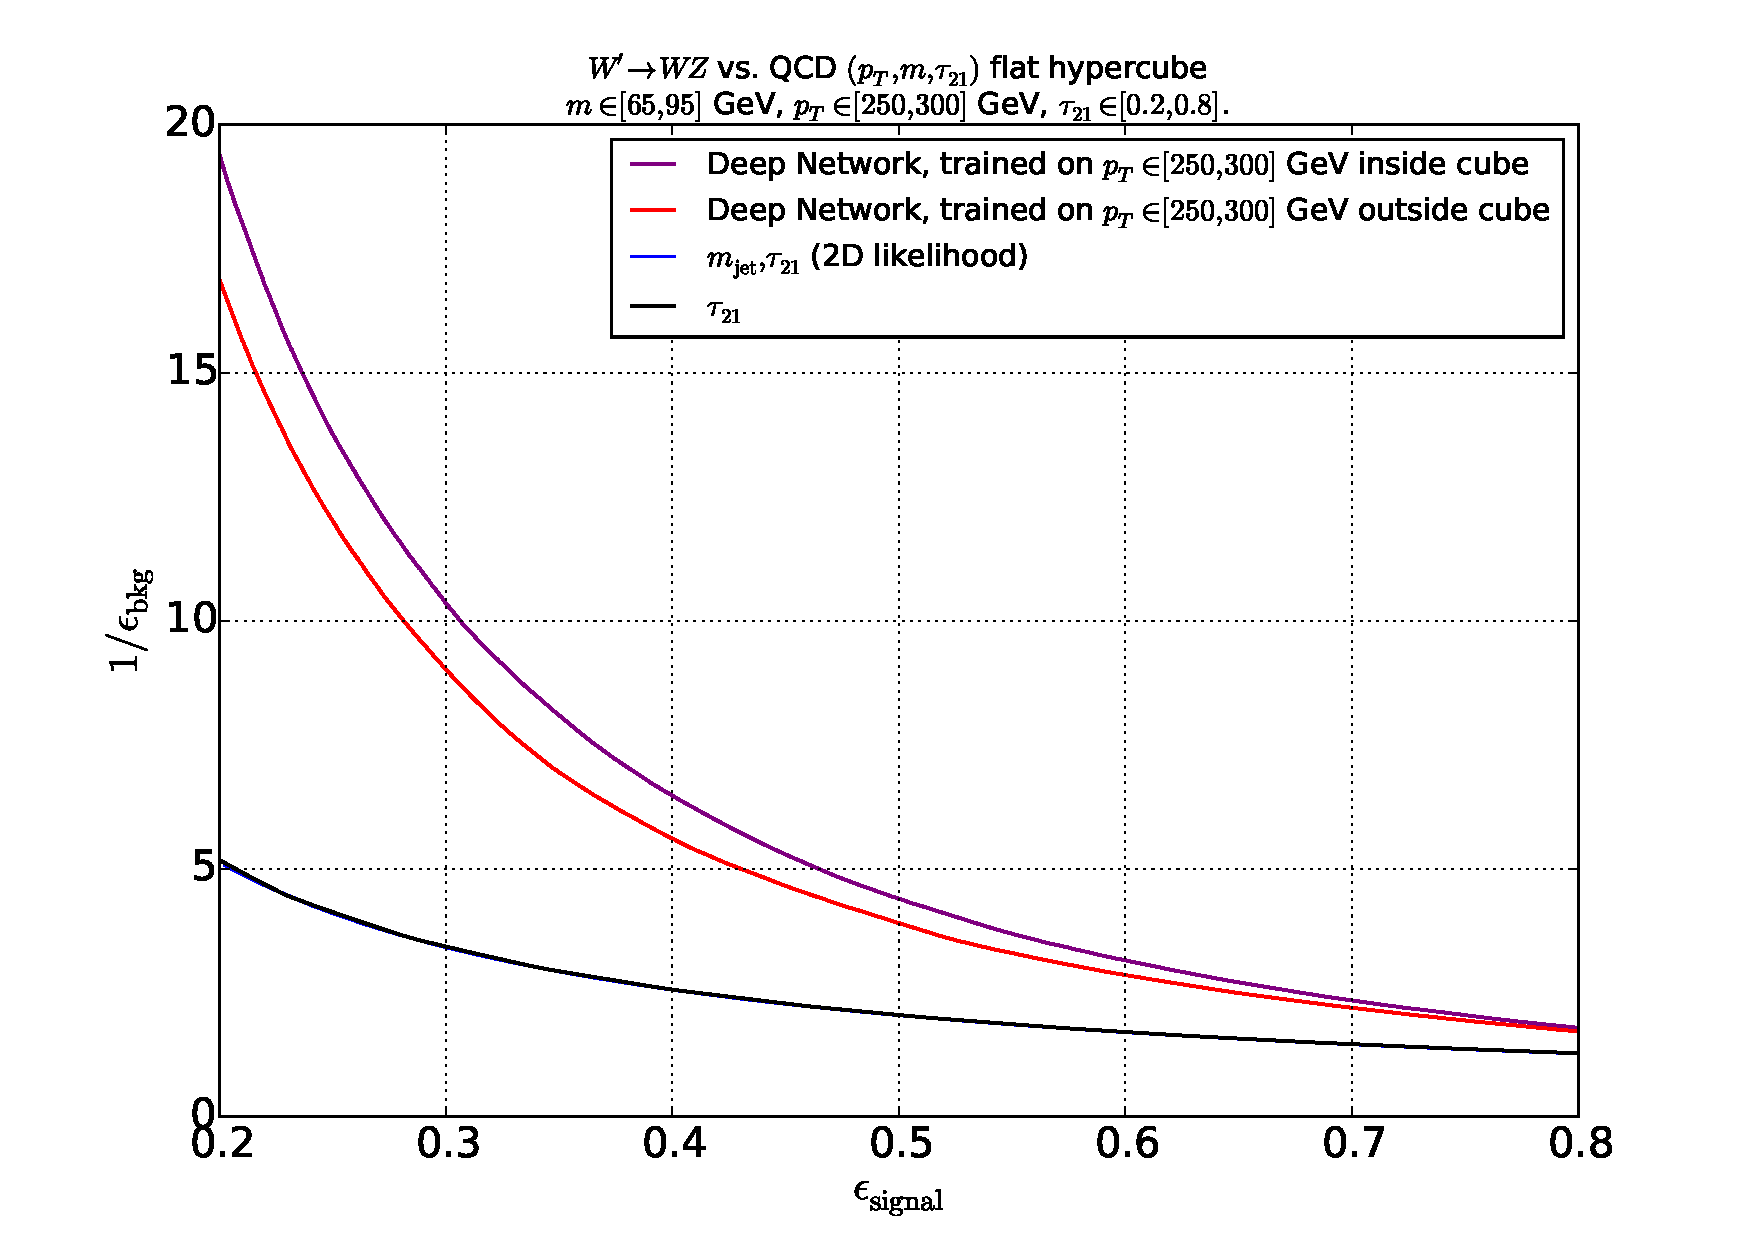
\includegraphics[width=0.95\textwidth]{figures/roc-cube-inside.pdf}
  \caption{ROC Curve for weigth-flattened hypercube, with $m\in[65, 95]\mathsf{GeV}$,  $p_T\in[250, 300]\mathsf{GeV}$, and  $\tau_{21}\in[0.2, 0.8]$}
  \label{fig:rocCube}
\end{figure}

% subsection flat_hypercube_studies (end)